\documentclass[tikz,border=2pt]{standalone}
\usepackage{amsmath,amssymb}
\usepackage{pgfplots}
\pgfplotsset{compat=1.18}

\begin{document}
% The first-success pmf with p = 0.3: the trial on which the first success occurs, so the
% support starts at k = 1 (it is the geometric distribution shifted by one).
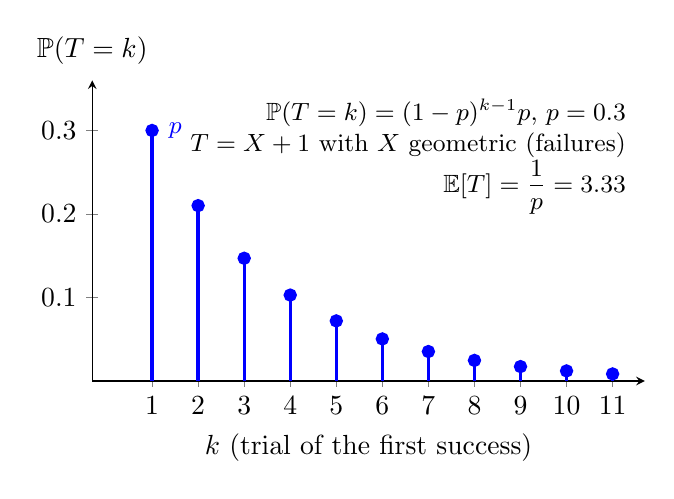
\begin{tikzpicture}
	\begin{axis}[
		axis lines=left, xmin=-0.3, xmax=11.7, ymin=0, ymax=0.36,
		xtick={1,...,11}, ytick={0.1,0.2,0.3},
		xlabel={$k$ (trial of the first success)}, ylabel={$\mathbb{P}(T=k)$}, ylabel style={rotate=-90, anchor=south, at={(axis description cs:0,1.02)}},
		width=8.6cm, height=5.4cm, clip=false
		]
		\addplot[ycomb, blue, very thick, mark=*, mark size=1.8pt] coordinates {(1,0.3000) (2,0.2100) (3,0.1470) (4,0.1029) (5,0.0720) (6,0.0504) (7,0.0353) (8,0.0247) (9,0.0173) (10,0.0121) (11,0.0085)};
		\node[anchor=north east, font=\small, align=right] at (axis cs:11.5,0.35) {$\mathbb{P}(T=k)=(1-p)^{k-1}p$, $p=0.3$\\ $T=X+1$ with $X$ geometric (failures)\\ $\mathbb{E}[T]=\dfrac1p=3.33$};
		\node[blue, anchor=west, font=\small] at (axis cs:1.15,0.3) {$p$};
	\end{axis}
\end{tikzpicture}
\end{document}
